\subsection{Entropy}

As a main motivation of why we need the term entropy, let's first look at the idea of \textbf{information gain}\sidenote{Information gain}. This can be applied to decision trees and asks for improvement in knowledge with each partitioning step, so better predictability of class labels in the nodes. This implies more homogenous interior nodes with every layer as visualized in the example in \ref{fig:3_information_gain}.

\begin{figure}[h]
  \centering
  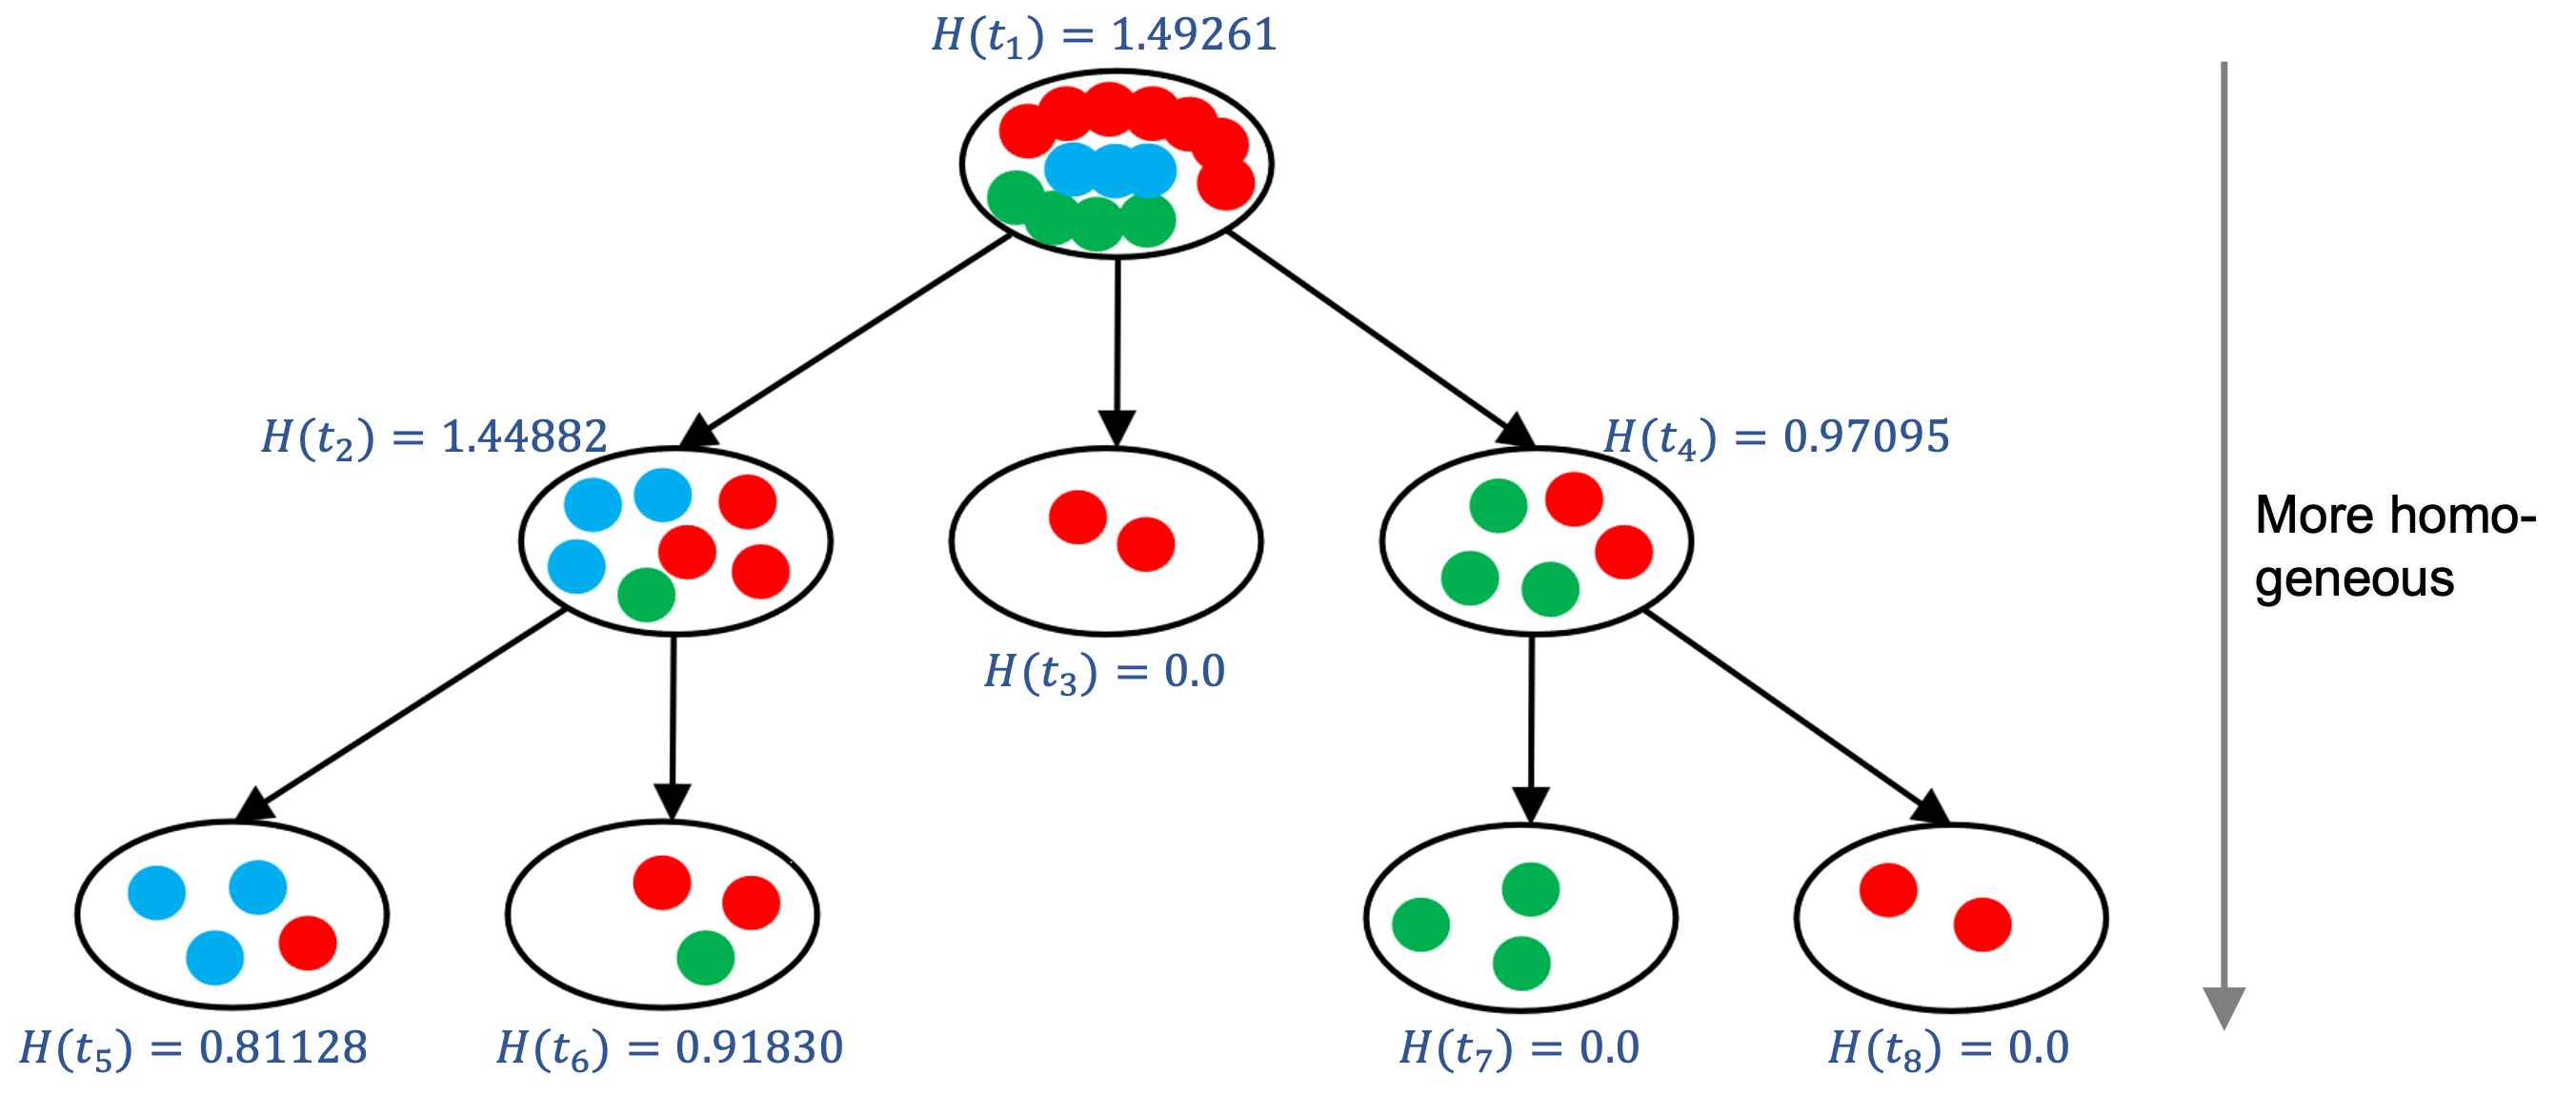
\includegraphics[width=0.9\textwidth]{assets/trees/entropy/entry_example.png}
  \caption{Idea of information gain and entropy intuition}
  \label{fig:3_information_gain}
\end{figure}

Next, we'll take a look into the intuition of the term \textbf{entropy}\sidenote{Entropy}. Figure \ref{fig:3_information_gain} also displays the entropy values. As one can see in the example:
\begin{itemize}
  \item Entropy \textbf{measures the impurity} in a set.
  \item With higher entropy, the \textbf{uncertainty in guessing} a class label grows.
  \item For a low entropy, the information gained when investigating the according data set is not very high, basically the data is "compressable". Entropy therefore also indicates \textbf{incompressibility}.
  \item Or put alternatively: entropy represents the number of bits needed to encode one instance knowing the population it comes from.
\end{itemize}

All of these statements are summarized in the formula:
\begin{align*}
  H(t) = - \sum_{i=1}^{n} \big( \Pr[t=i] \cdot \log_s (\Pr[t=i]) \big)
\end{align*}
The minus occurs, since $log_s(\frac{1}{x})=-\log_s(x)$. In this course, we will always take the logarithmic base $s=2$.

\begin{note}
For a better understanding, we will calculate the entropy for three example sets from figure \ref{fig:3_information_gain}.

\renewcommand{\arraystretch}{0.8}
\begin{tabular}{@{}>{\color{black}}p{0.4\textwidth} @{}>{\color{black}}p{0.6\textwidth}}
  \textbf{Example} & Distribution over colored dots\\
  \hline
  \textbf{1:} high entropy value &
  $n_{\text{red}}=7, n_{\text{blue}}=3, n_{\text{green}}=4$, so $n=14$ \\
  \multicolumn{2}{l}{$\implies H(t_1)=-\Big(
    \frac{7}{14} \cdot \log_2\left(\frac{7}{14}\right) + \frac{3}{14} \cdot \log_2\left(\frac{3}{14}\right) + \frac{4}{14} \cdot \log_2\left(\frac{4}{14}\right) 
  \Big) = 1.49261$} \\
  \textbf{2:} middle-high entropy value &
  $n_{\text{red}}=2, n_{\text{blue}}=0, n_{\text{green}}=3$, so $n=5$ \\
  \multicolumn{2}{l}{$\implies H(t_4)=-\Big(
    \frac{2}{5} \cdot \log_2\left(\frac{2}{5}\right) + \frac{2}{5} \cdot \log_2\left(\frac{2}{5}\right) 
  \Big) = 0.97095$} \\
  \textbf{3:} minimal entropy value & 
  $n_{\text{red}}=0, n_{\text{blue}}=0, n_{\text{green}}=3$, so $n=3$ \\
  \multicolumn{2}{l}{$\implies H(t_7)=-\Big(
    \frac{3}{3} \cdot \log_2\left(\frac{3}{3}\right) 
  \Big) = 0$}
\end{tabular}
\renewcommand{\arraystretch}{1}
\end{note}

Now that we have seen an example, we can easily see the \textbf{bounds of entropies}\sidenote{Bounds on $H$}.
\begin{itemize}
  \item The lowest possible entropy value yields when all instances have the same value, then $H(t) = 0$.
  \begin{itemize}
    \item Then there is no impurity at all, no uncertainty when guessing, and the information in the data is highly compressible.
  \end{itemize}
  \item The highest possible entropy value yields when we have an even distribution over all possible values, then $H(t) = - n \Big(\frac{1}{n}\cdot \log_2\left(\frac{1}{n}\right)\Big) = \log_2(n)$ is maximized
  \begin{itemize}
    \begin{note}\item E.g., for $3$ possible values: $log_2(3) \approx 1.58$\end{note}
    \item Then there is the highest possible impurity, highest uncertainty when guessing, and the information in the data is incompressible.
  \end{itemize}
\end{itemize}

Our goal when building decision trees is to have \textbf{pure leaves}, or the lowest possible average over the entropies of all leaves. With the entropy, we can now also put a number to the concept of information gain or loss, as can be seen in \ref{fig:3_information_gain_example}. When we have to select the next decision dividing an interior node, we select the features partitioning into groups with the least \textbf{remaining entropy} $rem$\sidenote{$rem$}, which is the weighted average over all subnodes.

\begin{figure}[h]
  \centering
  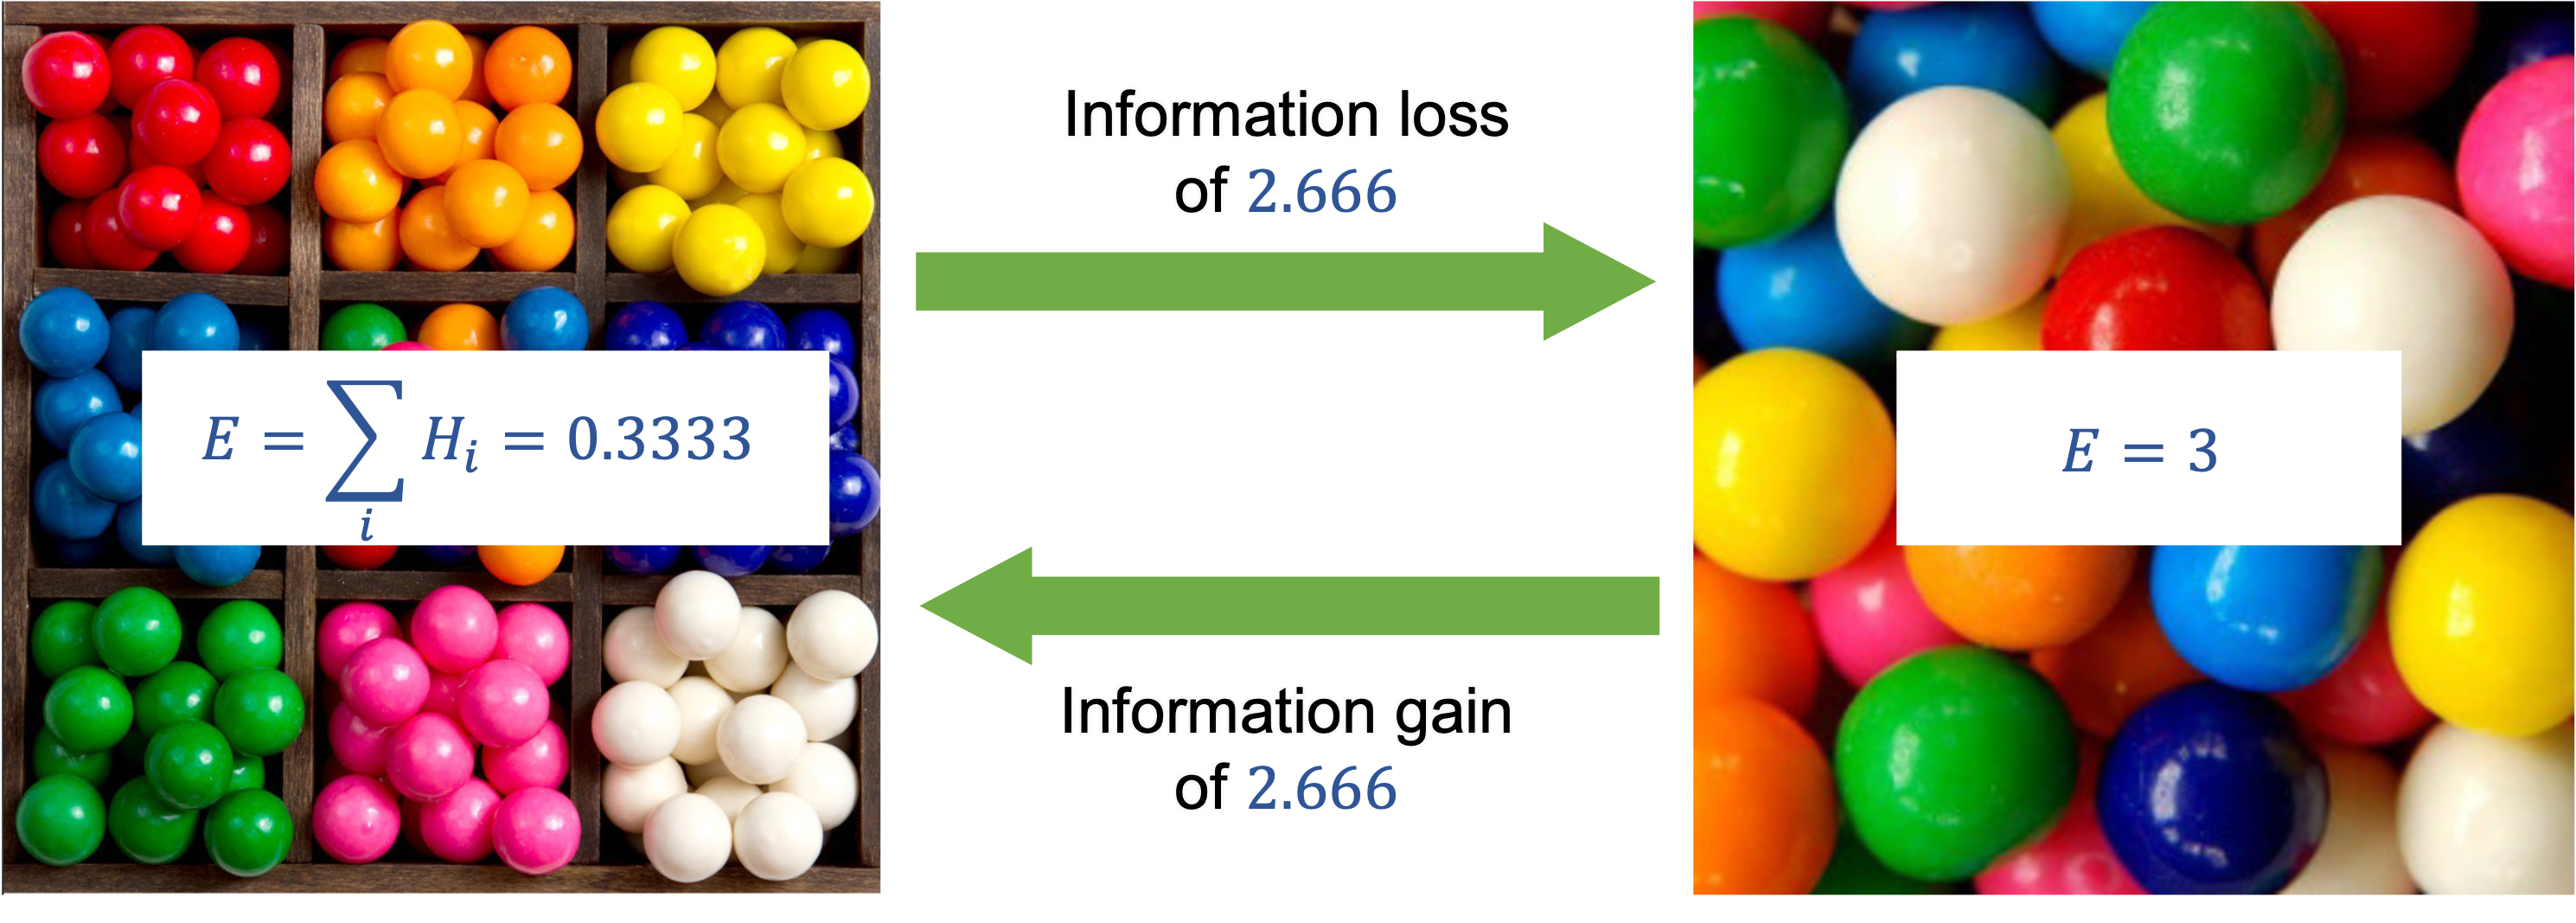
\includegraphics[width=0.7\textwidth]{assets/trees/entropy/loss_gain.png}
  \caption{Example for information gain and loss}
  \label{fig:3_information_gain_example}
\end{figure}
